\documentclass[10pt,stdletter]{newlfm}
%\newlfmP{addrfromleft,addrtoright,dateright,orderdatefromto,sigright,noLines}

\usepackage[english]{babel}   % English names on Introduction and other places
% \usepackage[norsk]{babel}   % Norwegian names on Introduction and other places
\usepackage[T1]{fontenc}        % Norwegian charset tegnsett (æøå)
\usepackage[utf8]{inputenc} % Norwegian charset
\usepackage{amsmath}
\usepackage{caption}
\usepackage{amssymb} %Comments here are fine
\usepackage{float}
\usepackage{lmodern}
\usepackage{parskip}
\usepackage{textcomp}
\usepackage{booktabs}
\usepackage{graphicx}

\usepackage{hyperref}
\hypersetup{
    colorlinks=true,
    linkcolor=blue, % Color of links in 'innholdsfortegnelse'
    filecolor=blue, % Doesn't show when colorlinks=true. It's the border-color.
    urlcolor=blue, % Links wil be nice blue color
}
\newcommand\tab[1][1cm]{\hspace*{#1}}

\usepackage{listings}
\lstset{basicstyle=\ttfamily,
  showstringspaces=false,
  commentstyle=\color{red},
  keywordstyle=\color{blue},
  escapeinside={(*@}{@*)},          % if you want to add LaTeX within your code
}


\begin{document}

\title{\textbf{LaTeX Article Template}}
\author{Author: Harald Lønsethagen}
% \date{\today}
\date{Last edited: \today\tab Version: 1.0}

\maketitle


% \clearpage\thispagestyle{empty}
\makeatletter
%\renewcommand\tableofcontents{\@starttoc{toc}}
%\makeatother
\tableofcontents
\newpage

\section{Introduction}
This is a template latex project ment to be used when creating new \LaTeX \space documents. You could easily copy this .tex file and delete all content, and then use what you need. I have included many examples of how you can use different features of \LaTeX, hopefully making it easy for you to get started.\\
\textbf{Pro tip:} type '\textbf{new\_latex}' in the terminal to generate a new latex project at your current working directory\footnote{This assumes you have installed \href{https://www.tug.org/texshowcase}{Linux Tricks}}.

\begin{lstlisting}[language=bash,caption={Example of getting started}]
harald@harald-tower:~$ cd ~/Documents/
harald@harald-tower:~/Documents$ new_latex
New LaTeX project name: test_project

Successfully generated new LaTeX project files in path:
/home/harald/Documents/2018-03-23_test_project_latex
\end{lstlisting}


\section{Links}
\href{www.vg.no}{This} is a link, which is clearly marked by the blue color. You can define the color in 'packages.tex'. You could link by doing like this: \url{www.vg.no}.
\newpage
\section{Figures}
Here you have a nice image of the universe in Fig. \ref{fig:universe}.
\begin{figure}[H]
    \centering
    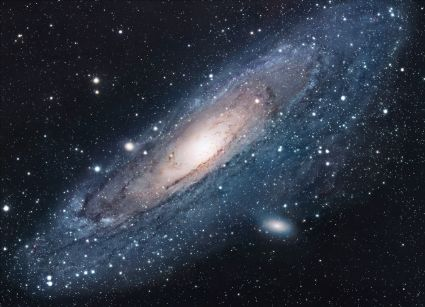
\includegraphics[scale=1.7]{universe}
    \caption{The Universe}
    \label{fig:universe}
\end{figure}

Getting a figure to be right where you want it can be a struggle.
I recommend using the 'H'-tag.

\section{Sections}
\subsection{Subsections}
This is what a subsection looks like and can be written as such:
\begin{lstlisting}
	\subsection{}
\end{lstlisting}
Check the .tex file to see how I can \textit{escape} LaTeX-commands,
\subsubsection{Subsubsections}
You can also make subsubsections.
\begin{lstlisting}
	\subsubsection{}
\end{lstlisting}
Is is \textbf{not} possible to make subsubsubsections.


\section{Textmodification}
You can change the font with simple commands.\newline{}
\begin{lstlisting}
	\textbf{Bold} (*@ $\rightarrow$ \textbf{Bold}@*)
\end{lstlisting}
\begin{lstlisting}
	\textit{Italic} (*@ $\rightarrow$ \textit{Italic}@*)
\end{lstlisting}
\begin{lstlisting}
	\textsc{Sc} (*@ $\rightarrow$ \textsc{Sc}@*)
\end{lstlisting}
\begin{lstlisting}
	\underline{Underline} (*@ $\rightarrow$ \underline{Underline}@*)
\end{lstlisting}
\begin{lstlisting}
	\emph{Emph} (*@ $\rightarrow$ \emph{emph}@*)
\end{lstlisting}
\begin{lstlisting}
	No commands (*@ $\rightarrow$ No commands@*)
\end{lstlisting}

\textbf{Ibsens ripsbærbusker og andre buskvekster, samt en djerv dvergbjerk}

\textit{Ibsens ripsbærbusker og andre buskvekster, samt en djerv dvergbjerk}

\underline{Ibsens ripsbærbusker og andre buskvekster, samt en djerv dvergbjerk}

\emph{Ibsens ripsbærbusker og andre buskvekster, samt en djerv dvergbjerk}

\section{Lists}
\subsection{Numbered lists}
\begin{enumerate}
	\item This is the first 'item' in the list
	\item You could have many items
	\item Just ramble along
	\item Tip: Don't use dot on the end of the line in a list
\end{enumerate}

\subsection{Bullet list}
\begin{itemize}
	\item This is the first \textit{item} in the bullet list
	\item If there is no reason to number a list, then use a bullet list
\end{itemize}

\subsection{Lists within a list}
\begin{itemize}
	\item Sometimes it is nice to have a list within a list
	\item This is still the first list
	\begin{itemize}
		\item This is an item in the list within a list
		\item Item 3.2
		\begin{itemize}
			\item A list within a list within a list
			\begin{itemize}
				\item This is the \textbf{deepest} level of lists within a list which is possible
			\end{itemize}
		\end{itemize}
	\end{itemize}
	\item Another item
	\begin{enumerate}
		\item It is possible to have a numbered list within a bullet list
		\begin{itemize}
			\item And to make a bullet list within a numbered list within a bullet list
		\end{itemize}
	\end{enumerate}
\end{itemize}

\section{Mathematical formulas}
\LaTeX \space is a fantastic tool for presenting mathematical formulas and calculations. It can take some while to get used to, but when you get over the initial bump, you can make your document look like \textbf{porn}.\cite{adams1995hitchhiker}
$$\cos (2\theta) = \cos^2 \theta - \sin^2 \theta$$
Next is an \textit{equation:}
\begin{equation}
\cos (2\theta) = \cos^2 \theta - \sin^2 \theta
\end{equation}

\begin{equation}\lim_{x \to \infty} \exp(-x) = 0\end{equation}

\begin{equation}\lim_{x \to \infty} \exp(-x) = 0\end{equation}

\begin{equation} \frac{n!}{k!(n-k)!} = \binom{n}{k}\end{equation}

\begin{equation} \displaystyle\sum_{i=1}^{10} t_i\end{equation}

\begin{equation} \int_0^\infty \mathrm{e}^{-x}\,\mathrm{d}x
\end{equation}

More \href{https://artofproblemsolving.com/wiki/index.php/LaTeX:Symbols}{\LaTeX \space symbols}.
% \begin{equation}
% ( a ), [ b ], \{ c \}, | d |, \| e \|,
% \langle f \rangle, \lfloor g \rfloor,
% \lceil h \rceil, \ulcorner i \urcorner
% \end{equation}

$$
\sum, \prod,	\coprod, \bigoplus, \bigotimes,	\bigodot, \bigcup, \bigcap,\biguplus,\bigsqcup,\bigvee,\bigwedge,\int,\oint,\iint[3],\iiint[3],\iiiint[3],\iiiint,\idotsint[3]
$$

$$
( a ), [ b ], \{ c \}, | d |, \| e \|,
\langle f \rangle, \lfloor g \rfloor,
\lceil h \rceil, \ulcorner i \urcorner
$$


% References
\bibliographystyle{plain}
\bibliography{references}

\end{document}
